In this section, we will discuss the results found in our research. First, we present a taxonomy that we created using the results from section~\ref{results}. This taxonomy can be useful to classify solutions of microservice performance and scalability.

After that, we perform a discussion about the results found in the reviewed articles. This discussion aims to presents what are the more often use to improve and analyze microservice applications related to scalability and performance. Finally, we show some tendencies in microservice implementations. 

\subsection{Taxonomy}
\begin{figure*}[htb]
\centering
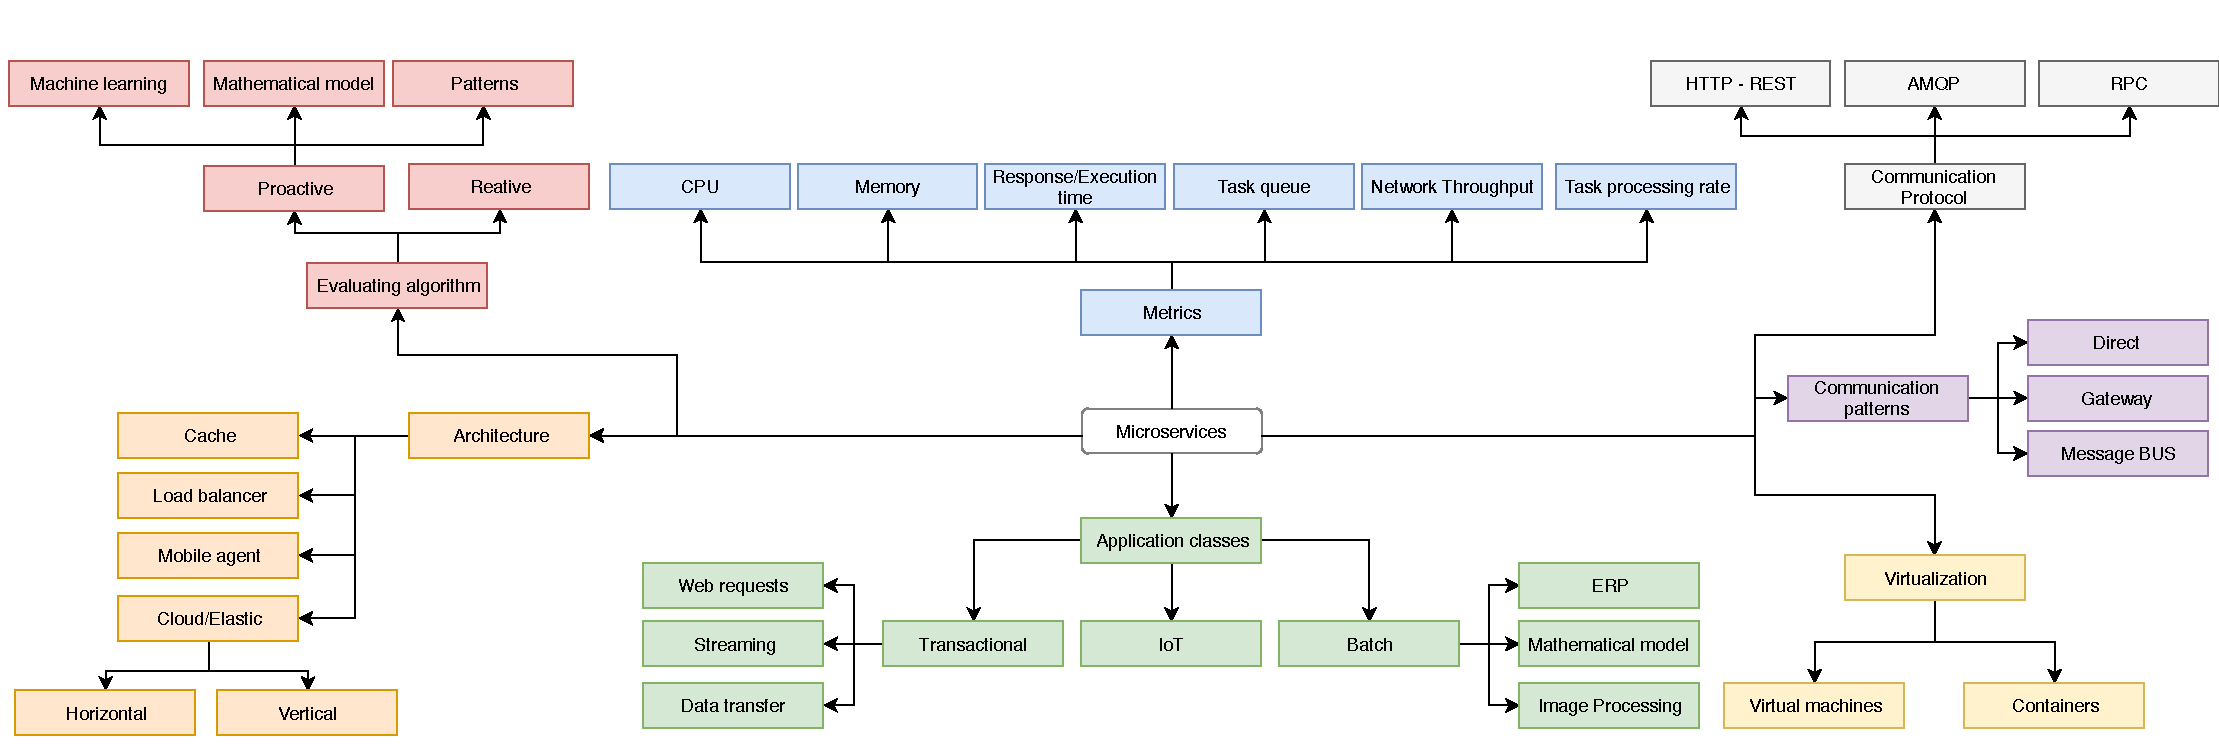
\includegraphics[scale=0.50]{Images/Taxonomy.pdf}
\caption{Microservice scalability and performance taxonomy. We divided into seven main groups: (a) Application classes, (b) Metrics, (c) Architecture, (d) Evaluating algorithm,  (e) Communication Protocol, (f) Communication Patterns, and (g) Virtualization.}
\label{taxonomy-figure}
\end{figure*}

Analyzing the results from the section~\ref{results}, we present the performance/scalability taxonomy from figure~\ref{taxonomy-figure}. In this section, we will present the classification, and in the next section, we will show how this classification appears in reviewed articles. We used seven main groups to describe how and when improvements in microservice performance and scalability appear. 

\subsubsection{Application classes}
First, we defined the application class of the microservice. It is essential to define the class of application because each class has a well determinate behavior and requirements. In the discussion, we will use this classification to related with the others research questions. We found in the reviewed articles three application classes main groups: (a) Internet of Things, (b) Transactional, and (c) Batch.

The Internet of Things (IoT) application class consists of applications with integration to sensors. A well-accepted architecture for IoT is EPCglobal~\cite{ArmenioJohnson2009The1.3}, and we will use to exemplifies microservice in IoT. This architecture has three main components: RFID readers, Application Level Events (ALE), and EPC Information Services (EPCIS). The RFID readers are the hardware layer that contains the sensors. The Application Level Events (ALE) is responsible for filtering and consolidate the sensor information. The last component is the EPC information service (EPCIS) that provides a service to access the data of readers. Microservice appears in ALE and EPCIS components. For example, EPCIS needs to scalable according to application requests.

The second application class is the transactional applications. Applications of this class usually have many application requests over the internet. We found three applications types in this class: Web Requests, Streaming, and Data Transfer. In Web Requests, the users request an internet address. The application performance is directly related to the amount of users requests. In a moment of the day, the system could have more requests than in others. In Streaming applications, the user receives many multimedia data. If the application lost some packages, the quality is not affected. Finally, the last transaction application is data transfer. In this type of application, the user requests some file and download this data from the server. Another application example is transfer files between two hosts.

The last application class is the batch applications. In this application class, the user executes one solicitation, and wait for the application ends. The application executes the data processing, that can take time. This application class is typically the class application used in high performance. We found three types of this class: Enterprise Resource Planning (ERP), Mathematical Model, and Image Processing. Enterprise Resource Planning (ERP) is the application to resolve some business issues. One example of ERP is ERP Payroll that needs to calculate the value to pay to the employees. The Mathematical Model try to resolve some not trivial mathematical problems. Some problems take some time to finalize. To finalize the problem in time, we can divide the problem in multiples microservices. Image processing application is applications that apply a change in some image. This application needs to apply a change in every image pixel, and this takes some time. Like the Mathematical Model, we can divide this problem in some microservices.

\subsubsection{Metrics}
Secondly, we classified the solutions by the metrics used in its analysis. This classification is essential to what metrics evaluate in applications. We found six metrics: (a) CPU, (b) Memory, (c) Response/Execution time, (d) Task queue, (e) Network Throughput, and (f) Task Throughput. The (a), (b), and (e) are metrics that can be measured directly in a host, while the others metrics are application metrics that needs some code instrumentation to be measured.

The first metric is the CPU that indicates the usage percentage from the Central Processing Unit. Usually, this metric shows system performance and the sum of work handled by the host. We will demonstrate in the discussion that this metric is widely used to analyze the performance.

Another widely used metric is memory utilization. This metric shows how much the application is retrieving data from physical to virtual memory and vice-versa. This paging can affect the performance because the CPU needs to stop the processing to manage the memory.

The Response/Execution time describes the metric how long the application or microservice takes to respond or finalize the processing. This metric directly indicates the microservice performance. For example, a microservice usually takes 5 minutes to finalize. At any time, this time grows to 10 minutes, so the microservice needs more resources.

The fourth metric is the task queue. Every microservice has a requisition queue that contains all microservice requisitions. An analyze in how this queue grows it is an essential metric to know how to adjust the microservice.

Another metric is the Network Throughput that shows the communication throughput in a system. According to an application grows, the microservice grows and have more communication. So, the Network Throughput affects the whole application performance.

The last metric is the task processing rate. This metric shows the number of jobs processed per time. For example, this can indicate that a microservice process five jobs per second. This metric directly shows the microservice performance.

\subsubsection{Architecture}
The third group is the architecture used to improve the microservice application. In this group, we found four architecture. 

The first is the cache based architecture that improves the microservice using a cache to avoid reprocessing the requests. This architecture is particularly useful in database microservices that perform a lot read actions. 

The second architecture is the load balancer. This architecture implements a load balancer that finds the better microservice node to process the incoming request. We found two ways to determine the better node to process a request: (a) On the fly decision and (b) define each node computation capacity. In (a) the load balancer defines on the fly which node will compute the incoming request based on the current workload of each node of the microservice application. This way is not an easy task to do on the fly and can affect the application performance. In (b) the system evaluates the computation capacity of each node. The system sends a simple request to each node and saves a node metric (e.g. response time). The load balancer used this metric to make a decision.

The third architecture is the mobile agent. This architecture involves an agent that migrates to the hosts. The agent migrates to a host to evaluate the current state of this host and to make adjustments aiming to improve the host performance.

Finally, the last architecture is the cloud. The previous architecture can use the cloud but does not use the high cloud differential: elasticity. For this reason, we created this group. When we discuss the reviewed articles, we will present how vital is elasticity to microservice, because of the cloud using elasticity is the most used architecture for microservice. Elasticity has two methods: (a) Horizontal and (b) Vertical.  In (a) the cloud adds or removes nodes and in (b) the cloud increases or decreases nodes resources. We described the elasticity in section~\ref{background} already.

\subsubsection{Evaluating algorithm}
The next group is the evaluating algorithm. This group describes how the system evaluates the metrics to perform actions. First, we divided into two algorithms: (a) Reactive and (b) Proactive. 

In (a) the system reacts to a change or collects metrics when a threshold reaches. For example, the system performs an action when the CPU of a node reaches 80\%. The reactive form has an easier implementation than the proactive, but this form can impact in the application performance. Could be too late for the application act just when a threshold reaches. Besides that, the application can be in an invalid state for a while. 

In (b) the system predicts when acting. Differently from reactive form, in the proactive form, the system collects metrics and predicts before an invalid state reaches. This algorithm is not too easy to implements, comparing to the reactive form. We found three proactive algorithms: Machine Learning, Mathematical Model, and Pattern Analysis. 
In the first proactive form, the system uses a machine learning algorithm, e.g. Support Vector Regression and Neural Networks, to predict metrics. Usually, machine learning algorithms need a period to learn before starting to predict. This requirement is a drawback of this approach.

Another proactive algorithm is the Mathematical Model. In this approach, the system uses an algorithm, such as Autoregressive Moving Average (ARMA) and Autoregressive Integrated Moving Average (ARIMA), to predict metrics. While machine learning needs a reasonable period for learning, Mathematical models start to predict as soon as possible. However, mathematical models have a less accurate output and minor outlier tolerance. 

The last proactive algorithm is the Patterns Analysis. In this approach, the system tries to match the current state of the application with to some defined pattern. If the match occurs, the system act. This approach is one of the most challenging algorithms to apply in a system to evaluate performance and scalability to microservices, comparing with machine learning and the mathematical model. Real applications can have values variations that the analysis need consider.

\subsubsection{Communication Protocol}
According the application grows, the quantity of microservice grows, and them needs to communicate with each other. So, the communication protocol affects the microservice performance. We found three protocols: (a) HTTP - Rest, (b) AMQP, and (c) RPC. 

The first protocol is the HTTP - Rest. This protocol provides interoperability between internet system. Usually, the microservices implement web service Restful. The second protocol is AMQP (Advanced Message Queuing Protocol) that implements a queue message protocol. Finally, the last protocol is the RPC (Remote Procedure Call). This protocol allows a procedure to execute in a different address space. 

\subsubsection{Communication Patterns}
As explained in the background section, there are three microservice communication patterns: (a) Direct, (b) Gateway, and (c) Message BUS.

In the Direct Communication, the microservices communicate between themselves directly and without any layer between the components. This pattern has a simpler implementation comparing with others patterns.

The second pattern is the Gateway. In this implementation, each microservice has a gateway that translates the different communication protocols. Besides that, this gateway can router when a microservice has some replicas.

The last pattern is the Message BUS. This pattern has a Message BUS that centralizes all requests to microservices. This Message BUS is a native router implementation because the first node to finalize takes another task from Message BUS.  

\subsubsection{Virtualization}
The last classification is the virtualization. This classification shows the virtualization level used in the microservice application. We found two virtualizations: (a) Virtual Machines and (b) Containers.

Virtual Machines (VMs) was the main virtualization type until recently. VMs are virtualization of a computer environment that allows the same functions that a real computer. A VM is isolated from the computer host. A node can host such VMs as its resources allow.

Such as VMs, Containers are an isolated and virtual computer environment. While each VM runs an entire operating system, each operating system runs several Containers. Containers are more lightweight than VMs.